\documentclass[norsk,a4paper,12pt]{article}
\usepackage[utf8]{inputenc}
\usepackage{graphicx} %for å inkludere grafikk
\usepackage{verbatim} %for å inkludere filer med tegn LaTeX ikke liker
\usepackage{tabularx}
\usepackage{booktabs}
\usepackage{amsmath}
\usepackage{float}
\usepackage{color}
\usepackage{listings}
\usepackage{hyperref}
\usepackage{amsmath}
\usepackage{tikz}

\lstset{language=c++}
\lstset{basicstyle=\small}
\lstset{backgroundcolor=\color{white}}
\lstset{frame=single}
\lstset{stringstyle=\ttfamily}
\lstset{keywordstyle=\color{red}\bfseries}
\lstset{commentstyle=\itshape\color{blue}}
\lstset{showspaces=false}
\lstset{showstringspaces=false}
\lstset{showtabs=false}
\lstset{breaklines}
\lstset{postbreak=\raisebox{0ex}[0ex][0ex]{\ensuremath{\color{red}\hookrightarrow\space}}}
\usepackage{titlesec}

\setcounter{secnumdepth}{4}
\usetikzlibrary{through,calc,er,positioning}

\titleformat{\paragraph}
{\normalfont\normalsize\bfseries}{\theparagraph}{1em}{}
\titlespacing*{\paragraph}
{0pt}{3.25ex plus 1ex minus .2ex}{1.5ex plus .2ex}


\title{FYS4411 - Computational Physics II\\\vspace{2mm} \Large{Project 1}}
\author{\large Dorthea Gjestvang\\ Even Marius Nordhagen}
\date\today
\begin{document}

\maketitle

\begin{itemize}
\item Github repository containing programs and results: \\\url{https://github.com/evenmn/FYS4411/tree/master/Project%201}
\end{itemize}

\begin{abstract}
This project aims to simulate a trapped Bose gas using Variational Monte Carlo (VMC) with both the  brute force Metropolis and the Metropolis-Hastings algorithms. Using a trial wave function with either spherical or elliptical harmonic oscillator (HO) potential, with and without a hard sphere potential, we calculate the ground state energy and onebody density for different numbers of particles. \textcolor{red}{The results are benchmarked with earlier publications.} \par 

Using the spherical HO with no interaction, both the brute force and the Metropolis-Hastings methods reproduces analytical calculations. Though the Hastings algorithm is slightly slower, it has a higher acceptance rate for the proposed moves in the VMC simulation. The onebody density distribution changes shape when introducing the hard sphere potential. \textcolor{red}{The system behaves as expected, and our results reproduces the benchmarks.}
\par 

\end{abstract}

\newpage

\section{Introduction}

In this project, we study the Bose-Einstein condensation (BEC) of a dilute gas of $^{87}$Rb atoms trapped in an elliptical harmonic oscillator. Bose-Einstein condensation occurs when atoms are cooled towards absolute zero, as they start occupying the same quantum state \cite{JE2016}. Even though the effect was predicted already in 1924, it was first observed by Anderson et.al. in 1995, which caused an immense interest in the subject \cite{SP}, \cite{Anderson}.

Our goal is to find an upper bound limit of the ground state energy for a system of a various number of particles, using an ansatz where the total wave function is a product of single particle wave functions. The Gross-Pitaevskii equation is applied to obtain an analytical energy approximation, which works as a benchmark for the energy. The theoretical framework is presented in section \ref{Theory}. \par

The main technique we will use is the variational Monte Carlo (VMC) method with two different Metropolis algorithms, presented in section \ref{Method}. To achieve the optimal trial wave function we vary the variational parameter $\alpha$ using the gradient descent method. In section \ref{Results} the upper bound energy is presented with the optimal wave functions and the onebody density. In section \ref{Discussion} we discuss our results, and compare them to results obtained from the articles found at \cite{DuBois}, \cite{Nilsen} and \cite{Dalfovo}.


\section{Theory} \label{Theory}

\subsection{Presentation of potential and trial wavefunction} 

We study a system of $N$ bosons trapped in a harmonic oscillator with the Hamiltonian given by 
\begin{equation}
\hat{H}=\sum_i^N\bigg(-\frac{\hbar^2}{2m}\nabla_i^2+V_{ext}(\vec{r}_i)\bigg)+\sum_{i<j}^NV_{int}(\vec{r}_i,\vec{r}_j)
\label{eq:Hamilton}
\end{equation}
with $V_{ext}$ as the external potential, which is the harmonic oscillator potential defined in equation \ref{eq:V_ext}, and $V_{int}$ as the interaction term, defined in equation \ref{eq:V_int}, which ensures the particles to be separated by a distance $a$. $\hbar$ is the reduced Plancks constant and $m$ is the mass of the particles in question. In this project we study the gas of $^{87}$Rb alkali atoms, which have a scattering length $a_{\text{Rb}}=0.0043$ given in units of a typical trap size $a_{HO}$. We will consider a harmonic oscillator which can either be spherical (all dimensions have the same scales) or elliptical (the vertical dimension has a different frequency from the horizontals).
\begin{equation}
\label{eq:V_ext}
V_{ext}(\vec{r})=
\begin{cases} 
   \frac{1}{2}m\omega_{HO}^2\vec{r}^2 & \text{(Spherical)} \\
   \frac{1}{2}m[\omega_{HO}^2(x^2 + y^2) + \omega_z^2z^2] & \text{(Elliptical)}.
\end{cases}
\end{equation}
where $\omega_{HO}$ is the frequency of the spherical harmonic oscillator and $\omega_z$ is the frequency of the elliptical trap in z-direction. 
\begin{equation}
\label{eq:V_int}
V_{int}(\vec{r}_i, \vec{r}_j)=
\begin{cases} 
0 & \text{if}\quad |\vec{r}_i-\vec{r}_j| \geq a \\
\infty & \text{if}\quad |\vec{r}_i-\vec{r}_j| < a
\end{cases}
\end{equation}
The trial wavefunction is on the form 
\begin{equation}
\Psi_T(\vec{r}_1, \vec{r}_2, ..., \vec{r}_N, \alpha, \beta)=\prod_i^Ng(\alpha, \beta, \vec{r}_i)\prod_{i<j}f(a,r_{ij})
\label{eq:WF}
\end{equation}
where $r_{ij}=|\vec{r}_i-\vec{r}_j|$ and $g$ is assumed to be a gaussian function,
\begin{equation}
g(\alpha, \beta, \vec{r}_i)=\exp[-\alpha(x_i^2+y_i^2+\beta z_i^2)],
\end{equation}
which is practical since
\begin{equation}
\prod_i^Ng(\alpha, \beta, \vec{r}_i)=\exp\Big[-\alpha\sum_{i=1}^N(x_i^2+y_i^2+\beta z_i^2)\Big].
\end{equation}
$\alpha$ is a variational parameter that we later use to find the energy minimum, and $\beta$ is a constant. The trial wave function used is the exact ground state wave function for a spherical harmonic oscillator with no interaction, so by choosing the correct $\alpha$, we will find the exact ground state energy. The $\alpha$ for the ground state wave function in this case is known to be $0.5$. The $f$ presented above is the correlation wave function, which is 
\begin{equation}
\label{eq:WF_interaction_part}
f(a,r_{ij})=
\begin{cases} 
   0 & r_{ij} \leq a \\
   \left(1-\frac{a}{r_{ij}}\right) & r_{ij} > a.
\end{cases}
\end{equation}
where $a$ is a parameter describing the minimum distance allowed between particles in the trap. This is also denoted as the Jastrow factor, and sets the wave function to zero when the distance between to particles are smaller than $a$, which that they will not contribute to the energy. 

\subsection{Local energy $E_L$ calculation}
In general we can find the energy of a system with a known wave function by solving the integral
\begin{equation}
E=\langle H\rangle = \frac{\int\psi^*(\vec{r})H\psi(\vec{r})d\vec{r}}{\int\psi^*(\vec{r})\psi(\vec{r})d\vec{r}}
\label{eq:general_energy}
\end{equation}
which depends on $|\psi(\vec{r})|^2$ only. This implies that sampling points from the $|\psi|^2$ distribution corresponds to sampling from the integrand $\psi^*H\psi$. We are in a situation where we do not know the exact wavefunction, and need to sample from the trial wave function in equation \ref{eq:WF}, which will probably not give us the exact energy. However, as we move the wave function closer to the true ground state wave function using the Metropolis algorithm (see section \ref{sec:Metropolis}), the computed energy (denoted local energy) should approach the ground state energy \cite{JKNilsen}. The algorithm used to conduct the Monte Carlo integration is presented in section \ref{VMC}.

For simplicity we use an expression for $E_L$ obtained from Schr\"{o}dinger's equation that let us avoid calculating the denominator in equation \ref{eq:general_energy},

\begin{equation}
E_L(\vec{r})=\frac{1}{\Psi_T(\vec{r})}\hat{H}\Psi_T(\vec{r}).
\label{eq:Local_energy}
\end{equation}
When the repulsive interaction is ignored ($a=0$), it can be shown that the local energy for a system of $N$ particles and $dim$ spatial dimensions is given by
\begin{equation}
E_L=dim\cdot N\cdot \alpha + \Big(\frac{1}{2}-2\alpha^2\Big)\sum_i\vec{r}_i^2,
\end{equation}
which is proven in appendix A. This is only true for the a spherical harmonic oscillator trap, for the elliptical trap we need to add $\beta$ in front of the z-component. You may also notice that this equation is scaled, more about that in section \ref{sec:scaling}.

For the a spherical harmonic oscillator where particle interactions are ignored, the analytical expression for the energy is well-known and reads $E = \hbar\omega(n + dim/2)$ where $n$ is the energy level and $dim$ is number of spatial dimensions. In this project we will study the ground state only, such that $n=0$, and for $N$ particles and $dim$ spatial dimensions we therefore obtain the expression for the ground state energy shown in equation \ref{eq:Energy_exact}.

\begin{equation}
E = \frac{1}{2}N\cdot dim\cdot\hbar\omega_{HO}.
\label{eq:Energy_exact}
\end{equation}


For $a\neq0$ it gets rather more complicated, because the Jastrow factor from equation \ref{eq:WF_interaction_part} is now different from 1. We also need to add the interaction term $V_{int}$, the hard-sphere potential from equation \ref{eq:V_int}. We are now ready to find an analytical expression for the local energy. By defining
\begin{equation}
f(a, r_{ij})=\exp{\bigg(\sum_{i<j}u(r_{ij})\bigg)}
\end{equation}
and doing a change of variables
\begin{equation}
\frac{\partial}{\partial \vec{r}_k}=\frac{\partial}{\partial \vec{r}_k}\frac{\partial r_{kj}}{\partial r_{kj}}=\frac{\partial r_{kj}}{\partial \vec{r}_k}\frac{\partial}{\partial r_{kj}}=\frac{(\vec{r}_k-\vec{r}_j)}{r_{kj}}\frac{\partial}{\partial r_{kj}}
\end{equation}
one will end up with
\begin{align}
E_L=\sum_k\Bigg(-\frac{1}{2}\bigg(4\alpha^2\Big(x_k^2+y_k^2+\beta^2z_k^2-\frac{1}{\alpha}-\frac{\beta}{2\alpha}\Big)
-4\alpha\sum_{j\neq k}(x_k, y_k, \beta z_k)\frac{(\vec{r}_k-\vec{r}_j)}{r_{kj}}u'(r_{kj})\notag\\
+\sum_{ij\neq k}\frac{(\vec{r}_k-\vec{r}_j)(\vec{r}_k-\vec{r}_i)}{r_{ki}r_{kj}}u'(r_{ki})u'(r_{kj})
+\sum_{j\neq k}\Big(u''(r_{kj})+\frac{2}{r_{kj}}u'(r_{kj})\Big)\bigg)+V_{ext}(\vec{r}_k)\Bigg) + V_{int}.\notag
\label{EL_total}
\end{align}
which is also shown in appendix A. This is not a pretty expression, but will yield correct results for both the interacting and non-inteacting case.



\subsubsection{Numerical calculation of $E_L$} \label{Numerical_calc_E_L}

Another approach when calculating $E_L$ is to split up the local energy expression as shown in equation \ref{eq:EL_num}, and calculate the local energy with a numerical approach where the second derivative needed to kind the kinetic energy can be approximated by the three-point formula, see equation \ref{eq:num_derv}.
\begin{equation}
\label{eq:EL_num}
E_{L,i}=-\frac{\hbar^2}{2m}\frac{\nabla_i^2\Psi_T}{\Psi_T}+V_{ext}(\vec{r}_i)=E_{k,i}+E_{p,i}
\end{equation}

\begin{equation}
\label{eq:num_derv}
f''(x)\simeq\frac{f(x+h)-2f(x)+f(x-h)}{h^2}.
\end{equation}
In our case the position is a three dimensional vector, so we need to handle each dimension separately. Both the analytical and the numerical local energy are implemented, and in section \ref{CPU}, the CPU time for the analytical and numerical approach are compared for various number of particles.
 

\subsubsection{Gross-Pitaevskii}
Since we study a dilute bose gas, we can use the Gross-Pitaevskii (GP) equation to estimate the energy density, also with interaction \cite{Gross}, \cite{Pitaevskii}. The energy is then given by an integral over all the positions (Ref.\cite{Nilsen}), 
\begin{equation}
E_{\text{GP}}[\Psi]=\int d\vec{r}\bigg[\frac{\hbar^2}{2m}|\nabla\Psi(\vec{r})|^2+V_{ext}(\vec{r})|\Psi|^2+\frac{2\pi\hbar^2a}{m}|\Psi|^4\bigg].
\label{eq:GP_integral}
\end{equation}
This integral can easily be solved analytically when we ignore the interaction (such that the Jastrow factor is one), and we get
\begin{equation}
E_{\text{GP}}(\alpha, \beta, N)=N\cdot\bigg(1+\frac{\beta}{2}\bigg)\bigg(\frac{1}{4\alpha}+\alpha\bigg)
\end{equation}
in three dimensions, which is derived in appendix D.

This is quite good for few particles and small hard-sphere diameter also with interaction, but since the average energy per particle should increase as we increase N, this will be more and more off. For the interacting case, we can solve the integral using a numerical method, for instance Monte Carlo integration. We will not implement this, but rather benchmark our results against the solution of GP when ignoring interaction.


\subsection{Onebody density} \label{sec:OB_theory}
In many cases it is convenient to know the positions of the particles, but when the number of particles increases, the set of positions turns into a messy collection of numbers which is not really informative ( in fact the exact positions can hardly be revealed according to Heisenberg's uncertainity principle). Instead of presenting the positions, the density of particles can give us a good overview of where the particles are located. With $N$ particles, the one-body density with respect to a particle $i$ is an integral over all particles but particle $i$:
\begin{equation}
\rho_i=\int_{-\infty}^{\infty}d\vec{r}_1\hdots d\vec{r}_{i-1}d\vec{r}_{i+1}\hdots d\vec{r}_N |\Psi(\vec{r}_1,\hdots \vec{r}_N)|^2.
\end{equation}
For the non-interacting case this integral can be solved analytically, as shown in equation \ref{eq:onebody}. Using Monte Carlo integration, the one-body density can be solved for any case. Anyhow, the interesting part is the radial density, so we either have to solve the integral in spherical coordinates or convert to spherical coordinates afterwards. 

Alternatively, the onebody radial density can be found in a more intuitive way. Imagine we divide the volume around particle $i$ into bins, where bin $j$ is located at a distance $j\cdot r_1$, as shown in figure 1. The radii are thus quantized. By counting the number of particles in a bin and dividing by the surface area, we find the average density of particles in the bin. If we decrease the initial radius $r_1$  of the innermost bin such that we have a large number of bins, this method can be used to find the onebody density. 
\begin{figure}[H]
	\centering
	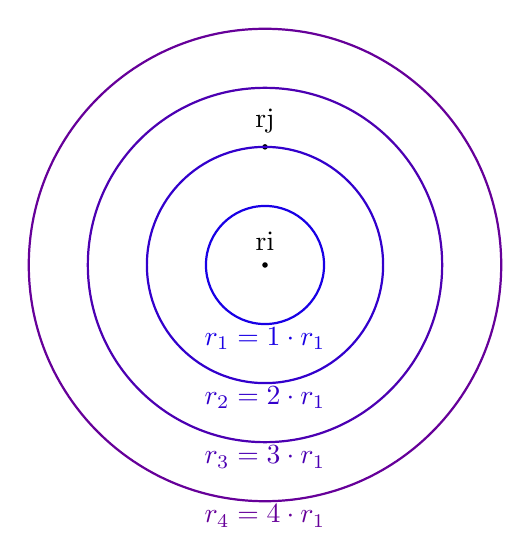
\begin{tikzpicture}[scale=0.50, thick, dot/.style={shape=circle,inner sep=+0pt, minimum size=+2pt, fill, label={#1}}]
       \coordinate[dot=ri] (ri) at (1,4);
       \coordinate[dot=rj] (rj) at (1,7);

       \foreach \cnt[count=\Cnt] in {.5, 1, 1.5, 2}
         \node[draw, color=red!\Cnt 0!blue, label={[inner sep=+1pt, red!\Cnt 0!blue]below:$ r_{\Cnt} = \Cnt\cdot r_1$}] at (ri) [circle through=($(ri)!\cnt!(rj)$)] {};
	\end{tikzpicture}
	\caption{One can find the onebody density by dividing the volume around a particle with coordinates $\vec{r}_i$ into bins and then count the number of particles, here illustrated in two dimensions.}
\end{figure}

The analytical expression without the Jastrow factor is found from \cite{DuBois}, and can be modified for our particular system, presented for the three dimensional case in equation \ref{eq:onebody}.
\begin{equation}
\rho_i=\frac{N\alpha\beta^{1/2}}{8\pi^{3/2}}e^{-r_i^2}.
\label{eq:onebody}
\end{equation}
Since the particles are identical the choice of the particle $i$ is of no consequence. 

\subsection{Scaling} \label{sec:scaling}
For big numerical projects, working with dimensionless quantities is a great advantage. Not only does it improve the code structure and performance, but it also avoids truncation errors due to small constants. For this project a natural scaling parameter for the energy is $\hbar\omega_{HO}$, which appears in the analytical energy expression in equation \ref{eq:Energy_exact}. The equivalent dimensionless equation can then be written as
\begin{equation}
E'=\frac{N\cdot dim}{2}
\end{equation}
where $E'=E/\hbar\omega_{HO}$. Additionally, we can scale the position with respect to the length of the spherical trap, $a_{HO}$, such that 
\begin{equation}
r_i'=\frac{r_i}{a_{HO}}=r_i\cdot\sqrt{\frac{m\omega_{HO}}{\hbar}},
\end{equation}
and the Hamiltonian turns into
\begin{equation}
H=\frac{1}{2}\sum_i\Big(-\nabla^2 + \vec{r}_i^2\Big)+\sum_{i<j}V_{int}(\vec{r}_i,\vec{r}_j)
\end{equation}
A watchful eye will see that this corresponds to setting $\hbar=\omega_{HO}=m=1$, which is the natural units. 

For the spherical trap situation we are left with the variational parameters $\alpha$ and $\beta$ only, but when we study an elliptical trap we still want to get rid of $\omega_z$. Since $\beta^2$ should be the factor in front of the z-coordinate when the Hamiltonian is dimensionless, it can be proven that $\beta=\omega_z/\omega_{HO}$, see appendix C. We end up with the Hamiltonian
\begin{equation}
H=\sum_i\bigg(\frac{1}{2}\Big(-\nabla^2 + x_i^2 + y_i^2 + \beta^2z_i^2\Big)\bigg)+\sum_{i<j}V_{int}(\vec{r}_i,\vec{r}_j)
\end{equation} 
where $\beta$ is chosen to be $\sqrt{8}\cong2.82843$, which was used in the experiment of Anderson et.al. \cite{Anderson}.

\subsection{Error estimation} \label{Error_estimation}
When presenting data from an experiment, one should always know the errors in the answer. Experimental data, including data from numerical experiments, are never determined beyond any doubt, and an estimate of this error should therefore be presented alongside the data. \par
There are two kinds of errors. Statistical errors originate from how much statistics one has; when $10^6$ measured points give approximately the same answer, one can be more sure that the actual value is close to those points, more so than if one only has 1 point of statistical data. Estimating the statistical error is easily done. The systematic error, however, is harder to handle. It arises for example from calculations being based on faulty theory, or defect measurement devices. Here, we will present how to get an estimate of the statistical error in a numerical experiment.
\par 
\vspace{3mm}
When conducting an experiment $\alpha$ with $n$ measured points, $ \{x_1, ..., x_n \}$, the sample mean $ \langle x_{\alpha} \rangle$ of the experiment  is defined as shown in equation \ref{eq:sample_mean}.

\begin{equation}
\label{eq:sample_mean}
\langle x_{\alpha} \rangle = \frac{1}{n} \sum_{k=1}^n x_{\alpha,k}
\end{equation}

The corresonding sample variance $\sigma_{\alpha}$ is then defined as

\begin{equation}
\sigma_{\alpha}^2 = \frac{1}{n} \sum_{k=1}^n (x_{\alpha,k} - \langle x_{\alpha} \rangle )^2
\end{equation}

This gives us the error in the given experiment $\alpha$. If we repeat this experiment $m$ times, the mean after all the experiments are

\begin{equation}
\label{eq:mean}
\langle x_{m} \rangle = \frac{1}{n} \sum_{k=1}^n  \langle x_{\alpha} \rangle.
\end{equation}

The total variance is then

\begin{equation}
\sigma_m^2 = \frac{1}{m} \sum_{\alpha=1}^m ( \langle x_{\alpha} \rangle - \langle x_{m} \rangle )^2.
\end{equation}

This can be reduced to 

\begin{equation}
\label{eq:sample_var_all_exp}
\sigma_m^2 = \frac{\sigma^2}{n} + \text{covariance term},
\end{equation}

where $\sigma$ is the sample variance over all the experiments, defined as 

\begin{equation}
\sigma^2 = \frac{1}{mn} \sum_{\alpha=1}^m \sum_{k=1}^n (x_{\alpha, k} - \langle x_m \rangle )^2
\end{equation}

and the covariance is the linear correlation between the measured points. The definition of the covariance is shown in equation \ref{eq:covariance}.

\begin{equation}
\label{eq:covariance}
cov(x,y) = \frac{1}{n^2} \sum_i \sum_{j >i} (x_i - x_j) (y_i - y_j).
\end{equation}

A common simplification is to reduce equation \ref{eq:sample_var_all_exp} to the following:

\begin{equation}
\label{eq:variance_simplified}
\sigma^2 \approx \langle x^2 \rangle - \langle x \rangle^2
\end{equation}

This equation, however, does not take into account the covariance term from equation \ref{eq:sample_var_all_exp}, and as the covariance term is added to the expression for the variance, \ref{eq:variance_simplified} will underestimate the uncertainty $\sigma$ for positive covariances.

A direct implementation of equation \ref{eq:sample_var_all_exp} including the covariance term is not suitable, as the expression for the covariance includes a double sum, and for a large number of iterations, this will turn into an extremely time consuming process for a large number of Monte Carlo iterations. Luckily, there are methods for calculating an accurate estimation of the variance without including a double loop in the Monte Carlo program. One of these methods is the blocking method, which is presented in section \ref{Blocking}.

\section{Method} \label{Method}
\subsection{Variational Monte Carlo}\label{VMC}
Variational Monte Carlo (VMC) is a widely used method for approximating the ground state of a quantum system. The method is based on Markov chains, where one particle or a set of particles are moved one step for each cycle, i.e.
\begin{equation}
\vec{R}_{new} = \vec{R} + r\cdot \text{step}.
\end{equation}
Both the direction and particles moves are randomly chosen, so with a plain VMC implementation the particles will move randomly and independently of each other. We are going to use the Metropolis algorithm in addition to the VMC, where the Metropolis algorithm accepts or rejects moves based on the probability ratio between the old and the new position. This makes the system approach the most likely state, and the idea is that after a certain number of cycles the system will be in the most likely state. 

\subsection{Metropolis Algorithm} \label{sec:Metropolis}
As mentioned above the task of the Metropolis algorithm is to move the system against the most likely state. The standard algorithm, here named brute force, is the simplest one, and does not deal with the transition probabilities. The modified Metropolis-Hastings algorithm includes, on the other hand, the transition probabilities and will be slightly more time consuming per cycle. We expect the latter to converge faster to the most likely state. 

The foundation of the Metropolis algorithm is that the probability for a system to undergo a transition from state $i$ to state $j$ is given by the transition probability multiplied by the acceptance probability
\begin{equation}
W_{i\rightarrow j} = T_{i \rightarrow j}\cdot A_{i \rightarrow j}
\end{equation}
where $T_{i \rightarrow j}$ is the transition probability and $A_{i \rightarrow j}$ is the acceptance probability. Built on this, the probability for being in a state $i$ at time (step) $n$ is
\begin{equation}
P_i^{(n)} = \sum_j\bigg[P_j^{(n-1)}T_{j \rightarrow i}A_{j \rightarrow i} + P_i^{(n-1)}T_{i \rightarrow j}(1-A_{i \rightarrow j})\bigg]
\end{equation}
since this can happen in two different ways. One can start in this state $i$ at time $n-1$ and be rejected or one can start in another state $j$ at time $n-1$ and complete an accepted move to state $i$. In fact $\sum_j T_{i \rightarrow j} =1$, so we can rewrite this as 
\begin{equation}
P_i^{(n)} = P_i^{(n-1)} + \sum_j\bigg[P_j^{(n-1)}T_{j \rightarrow i}A_{j \rightarrow i} - P_i^{(n-1)}T_{i \rightarrow j}A_{i \rightarrow j}\bigg].
\end{equation}
When the times goes to infinity, the system approaches the most likely state and we will have $P_i^{(n)} = p_i$, which requires
\begin{equation}
\sum_j\bigg[p_jT_{j \rightarrow i}A_{j \rightarrow i} - p_iT_{i \rightarrow j}A_{i \rightarrow j}\bigg]=0.
\end{equation}
Rearranging, we obtain the useful result
\begin{equation}
\frac{A_{j\rightarrow i}}{A_{i\rightarrow j}}=\frac{p_iT_{i\rightarrow j}}{p_jT_{j\rightarrow i}}
\end{equation}
which will be used in the acceptance criteria.

\subsubsection{Brute force}
In the brute force Metropolis algorithm we want to check if the new position is more likely than the current position, and for that we calculate the probabilities $P(\vec{R})=|\Psi_T(\vec{R})|^2$ for both positions. We get rid off the transition probabilities setting $T_{i\rightarrow j}=T_{j\rightarrow i}$, and then end up with the plain ratio
\begin{equation}
w=\frac{P(\vec{R}_{new})}{P(\vec{R})}=\frac{|\Psi_T(\vec{R}_{new})|^2}{|\Psi_T(\vec{R})|^2}.
\end{equation}
$w$ will be larger than one if the new position is more likely than the current, and smaller than one if the current position is more likely than the new one. Metropolis handle this by accepting the move if the ratio $w$ is larger than a random number $r$ in the interval $[0,1]$, and rejecting if not:
\begin{equation}
\text{New position: }
\begin{cases} 
   \text{accept} & \text{if}\quad w > r \\
   \text{reject} & \text{if}\quad w \leq r.
\end{cases}
\end{equation}

\subsubsection{Importance sampling} \label{Importance_sampling}
The importance sampling technique is often refered to as Metropolis-Hastings algorithm. The approach is the same as for the brute force Metropolis algorithm, but we will end ut with a slightly more complicated acceptation criteria. To understand the details, we need to begin with the Fokker-Planck equation, which describes the time-evolution of the probability density function $P(R,t)$. In one dimension it reads
\begin{equation}
\frac{\partial P(R,t)}{\partial t} = D\frac{\partial}{\partial R}\bigg(\frac{\partial}{\partial R} - F\bigg)P(R,t).
\end{equation}
where $F$ is the drift force given by equation \ref{eq:drift_force} and $D$ is the diffusion coefficient, in this case equal $0.5$. Calculations of the analytical expression of the drift force $F$ for a spherical harmonic oscillator and $a=0$ can be found in appendix B.

\begin{equation}
	\label{eq:drift_force}
	F(R) = \frac{2 \nabla \psi_T}{\psi_T}
\end{equation}
Even though the probability density function can give a lot of useful information, an equation describing the motion of a such particle would be more appropriate for our purposes. Fortunately this equation exists, and satisfies the Fokker-Planck equation. The Langevin equation can be written as
\begin{equation}
\frac{\partial R(t)}{\partial t}=DF(R(t)) + \eta
\end{equation}
where $\eta$ can be considered as a random variable. This differential equation can be solved by applying the forward Euler method and introducing gaussian variables $\xi$
\begin{equation}
R_{new} = R + DF(R)\Delta t + \xi\sqrt{\Delta t}
\end{equation}
which will be used to update the position. This is an improved way of choosing the direction in which the particle is moved compared to the brute force algorithm, as the drift force $F(R)$ says something about which direction the particle is pushed in, and the choice of the new proposed position is thus dependent on this.

Moreover we also need to update the acceptance criteria since we no longer ignore the transition probabilities. With the Fokker-Planck equation as base, the transition probabilities are given by Green's function
\begin{align}
T_{R\rightarrow R_{new}}&=G(R_{new},R,\Delta t)\notag\\
&=\frac{1}{(4\pi D\Delta t)^{3N/2}}\exp[-(R_{new} - R - D\Delta tF(R))^2/4D\Delta t] 
\end{align}
and the acceptance criteria becomes
\begin{equation}
r<\frac{G(R,R_{new},\Delta t)|\Psi_T(R_{new})|^2}{G(R_{new},R,\Delta t)|\Psi_T(R)|^2}.
\end{equation}



\subsection{Minimization methods}
When the interaction term is excluded, we know which $\alpha$ that corresponds to the energy minimum, and it is in principle no need to try different $\alpha$'s. However, sometimes we have no idea where to search for the minimum point, and we need to try various $\alpha$ values to determine the lowest energy. If we do not know where to start searching, this can be a time consuming activity. Would it not be nice if the program could do this for us?

In fact there are multiple techniques for doing this, where the most complicated ones obviously also are the best. Anyway, in this project we will have good initial guesses, and are therefore not in need for the most fancy algorithms. 

\subsubsection{Gradient descent}
Perhaps the simplest and most intuitive method for finding the minimum is the gradient descent method, which reads
\begin{equation}
\label{eq:GD}
\alpha^+=\alpha - \eta\cdot\frac{d\langle E_L(\alpha)\rangle}{d\alpha}.
\end{equation}
where $\alpha^+$ is the updated $\alpha$ and $\eta$ is the step size. The idea is that one finds the gradient of the energy with respect to a certain $\alpha$, and moves in the direction which minimizes the energy. This is repeated until one has found an energy minimum, where the energy minimum is defined as either where $\frac{d\langle E_L(\alpha)\rangle}{d\alpha}$ is smaller than a given tolerance, or the $\alpha$ energy fluctuates around a value, and thus changes minimally.
\par 
\vspace{3mm}

To implement equation \ref{eq:GD}, we need an expression for the derivative of $E_L$ with respect to alpha:

\begin{equation}
	\label{eq:E_L_der_wrt_alpha}
	\bar{E_{\alpha}} = \frac{d \langle E_L (\alpha) \rangle}{d \alpha}.
\end{equation}
By using the expression for the expectation value for the local energy $ \langle E_L (\alpha) \rangle$ in equation \ref{eq:exp_EL} 

\begin{equation}
	\label{eq:exp_EL}
	\langle E_L (\alpha) \rangle = \frac{ \langle \psi_T(\alpha) | H | \psi_T(\alpha)  \rangle}{ \langle \psi_T(\alpha)  |  \psi_T(\alpha)  \rangle }
\end{equation}
and applying the chain rule of differentiation, it can be shown that equation \ref{eq:E_L_der_wrt_alpha} is equal to equation \ref{eq:E_L_der_wrt_alpha_expression}

\begin{equation}
	\label{eq:E_L_der_wrt_alpha_expression}
	\bar{E_{\alpha}} = 2 \bigg[\langle E_L (\alpha)  \frac{ \bar{\psi_{\alpha}}}{\psi_{\alpha}}\rangle - \langle E_L (\alpha) \rangle \langle \frac{\bar{\psi_{\alpha}}}{\psi_{\alpha}} \rangle\bigg]
\end{equation}
where

\begin{equation}
	\bar{\psi_{\alpha}} = \frac{d \psi (\alpha)}{d \alpha}.
\end{equation}

The algorithm of this minimization method is thus as follows:

\lstset{basicstyle=\scriptsize}
\begin{lstlisting}

for(max number of iterations with minimizing)
	
	do M Monte Carlo cycles
	calculate E_L and dE_L/dalpha 
	
	Check if dE_L/dalpha < eps or alpha fluctuation over the last 5 steps is < eps
	
	
		if yes, print optimal alpha and break loop
		if no, continue to next iteration


\end{lstlisting}

\subsection{Blocking method} \label{Blocking}

As described in section \ref{Error_estimation}, we need a method to give a proper estimation of the variance $\sigma^2$ of the points in our experiment, preferably without calculating the double loop from the expression of the covariance in equation \ref{eq:covariance}. 
\par 
\vspace{3mm}

One method that can be used, is the blocking method, which is quite fast and can handle large data sets. Say that we have a data set $\{x_1, ...,x_i,..., x_n\}$ from an experiment, which in our case will be the estimations of the local energies for each Monte Carlo cycle. The mean of this data set is $m$, and we want to estimate the variance of this data set, $\sigma^2 (m)$, including the covariance.

The variance is defined as 

\begin{equation}
	\sigma^2 = \frac{1}{n-1} \sum_i (x_i - m)
\end{equation}
However, this does not include the covariance, as the points $x_i$ are correlated.

If we transform the data set $\{x_1, ...,x_i,..., x_n\}$ by taking the mean of two neighbouring points in the following way
\begin{equation}
	x'_i = \frac{1}{2}(x_{2i} + x_{2i+1})
\end{equation}
the number of points in the transformed data set $n' = \frac{1}{2} n$. Each pair of points $x'_i$ is referred to as a block, and using the variance formula above, the variance within each block is calculated. An estimate of the total variance $\hat{\sigma}$ is then
 
 \begin{equation}
 \hat{\sigma} = \frac{\sigma_1 + ... + \sigma_{n'}}{n'}
 \end{equation}
 
By repeating this procedure several times, and each time using more measurements for each block, the estimated standard deviation $\hat{\sigma}$ will grow, and eventually reach a plateau. When the estimated standard deviation $\hat{\sigma}$ flats out, it means that the blocks are no longer correlated, and thus the covariance which bugged us in equation \ref{eq:sample_var_all_exp}, is now 0. The covariance is therefore accounted for, and the $\hat{\sigma}$ is now a good estimation of the error in the data set.


\section{Code} \label{sec:code}
This project is much about developing the code to make VMC run correctly, and in this section we will explain briefly how the code works and which implementation techniques we use. The implementation is dimensionless, such that the variational parameters are the only quantities. 

\subsection{Code structure}
To keep the program neat, specific parts were placed in specific files. For instance, a file gd.cpp handle everything about the gradient descent method, and another file wavefunction.cpp (a little misleading) contains a class which both sets up the wave function and calculate the local energy given a wave function. We also collected the tools that are used by multiple scripts in its own file to maximize the reuse of the code, in particular Green's function and the quantum force calculations. In figure \ref{fig:code_structure} we give an overview of the implementation, where the lines indicate which scripts that communicate. 

\begin{figure}[H]
\centering
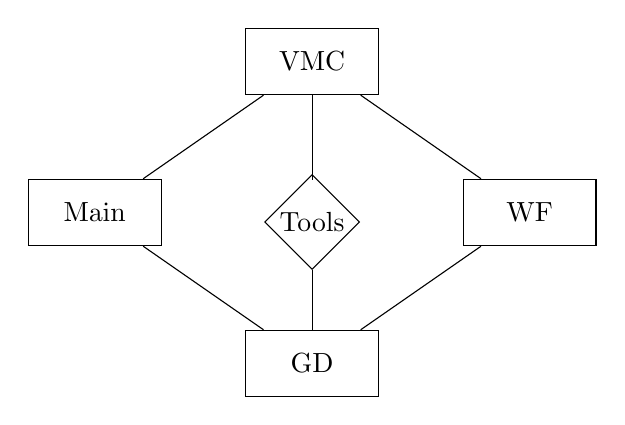
\begin{tikzpicture}[auto,node distance=1.5cm]
  \node[entity] (node1) {VMC}
    child {};
  \node[entity] (node2) [below right = of node1] {WF};
  \node[entity] (node3) [below left = of node1] {Main};
  \node[entity] (node4) [below right = of node3] {GD};
  \node[relationship] (rel1) [below=1cm of node1] {Tools};

  \path (node1) edge node {} (node2)
                edge node {} (node3)
                edge node {} (rel1);
  \path (node4) edge node {} (node2)
                edge node {} (node3)
                edge node {} (rel1);
\end{tikzpicture}
\caption{An overview of the code structure. metropolis.cpp is refered to as VMC, gd.cpp is GD, wavefunction.cpp is WF, tools.cpp is Tools and obviously main.cpp is Main. See text for furter description.}
\label{fig:code_structure}
\end{figure}
The acronyms are not really accurate, VMC is of course much about the Metropolis algorithm, and GD contains both the VMC and the Metropolis algorithm. Anyway, it is hard to find acronyms that tells everything about the script. A standard VMC run goes as following: metropolis.cpp (VMC) is called from main.cpp (Main), which agains calls wavefunction.cpp (WF) to set up the wave function, calls tools.cpp (Tools) to get the value of Green's function and the quantum force and then again calls WF to obtain the local energy. At the end the local energy is printed out.

\subsection{Implementation}
We use the vector package to create a 2D-array where the positions are stored. For the exact implementation, see the github repository linked on page one. We always struggle for better performance, and to achieve that we try to avoid heavy loops and repetition of calculations. A second priority is to make the code as general as possible, such that the code can be reused for other purposes. As an example we always loop over an arbitrary given number of dimensions, and similar operations are done throughout the programs. 

\subsubsection{VMC and Metropolis}
Present pseudo code of how VMC and Metropolis are implemented

\subsubsection{GD}

\subsubsection{Tests}



\section{Results} \label{Results}

We will first present the results obtained without repulsive interaction, and thoughout this part we will consequently use $\alpha=0.5$ and run for $1e6$ Monte Carlo cycles and for three spatial dimensions. 

Thereafter we will turn to the more realistic and interesting situation where the particles interact with each other. We will still study the behavior in three dimensions and for $1e6$ cycles, but we need to set the scattering distance to $a=0.0043$ and find the $\alpha$ which gives the minimum local energy. In this part we will also turn on the elliptical harmonic oscillator potential.

\subsection{$E_L$ as a function of the variational parameter $\alpha$}
In search of the energy minimum we tried various $\alpha$ values, and optimal $\alpha$ was 0.5, as one can see in figure \ref{fig:EL_as_func_of_alpha}. The variance associated with the energy measurement in figure \ref{fig:EL_as_func_of_alpha}, and we see that the energy minimum and the variance minimum share the same $\alpha$.

\begin{figure} [H]
	\centering
	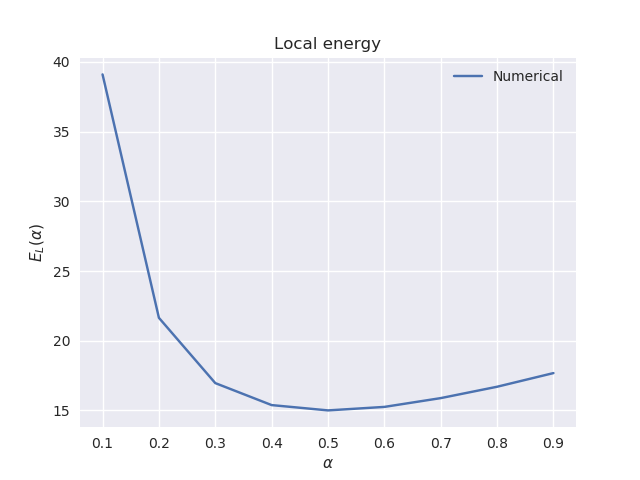
\includegraphics[scale=0.6]{images/energy.png}
	\caption{The local energy $E_L$ calculated with the brute force Metropolis algorithm, as a function of the variational parameter $\alpha$ in the interval $[0.1,0.9]$. for each $\alpha$ we used $1e6$ Monte Carlo cycles in three spatial dimensions.}
	\label{fig:EL_as_func_of_alpha}
\end{figure} 

\begin{figure} [H]
	\centering
	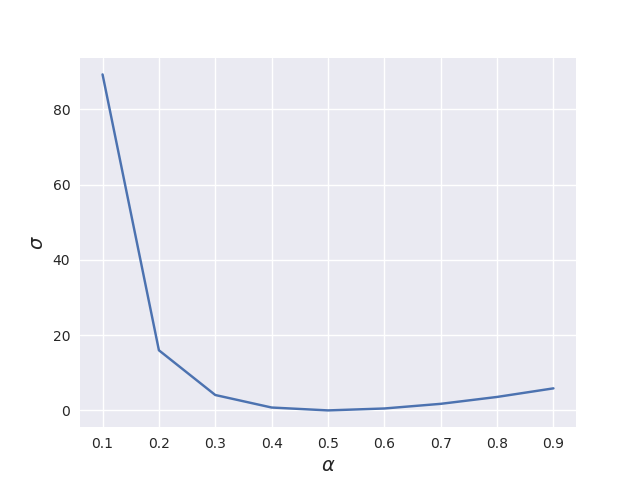
\includegraphics[scale=0.6]{images/variance.png}
	\caption{The variance of the local energy $E_L$ calculated with the brute force Metropolis algorithm, as a function of the variational parameter $\alpha$ associated with the energy plot in figure \ref{fig:EL_as_func_of_alpha}. The variance is calculated with equation \ref{eq:variance_simplified}}.
	\label{fig:variance_EL_as_func_of_alpha}
\end{figure} 

\subsection{$E_L$ calculation and CPU-time}\label{CPU}
For the brute force Metropolis algorithm we developed both an analytical and a numerical method to calculate the local energy. In table \ref{tab:BFmet} we present the results from these calculations and the performance. The results from the calculations with the Metropolis-Hastings algorithm are presented in table \ref{tab:ISmet}.

\begin{table} [H]
	\centering
	\caption{The local energy calculated for $a=0$  without hard-sphere interaction with brute force Metropolis algorithm, for both the analytical and numerical local energy calculation. The variational parameter $\alpha$ is $0.5$. The results are compared to the exact answer, obtained from equation \ref{eq:Energy_exact}. The number of Monte Carlo cycles is fixed to $M=1e6$, and the performance is presented along with the calculated energies. }
	\begin{tabularx}{\textwidth}{X|XX|XX|X} \hline
		\label{tab:BFmet}
		& \multicolumn{2}{X}{\textbf{Analytical}} & \multicolumn{2}{X}{\textbf{Numerical}} & Exact \\
		$N$ & $\langle E_L\rangle$ [$\hbar\omega_{HO}$] & CPU-time [s] & $\langle E_L\rangle$ [$\hbar\omega_{HO}$] & CPU-time [s]& $\langle E_L\rangle$ [$\hbar\omega_{HO}$]\\ \hline
		1 & 1.5000(15) & 0.15420 & 1.5000(15) & 0.65714 & 1.5000\\
		10 & 15.000(15) & 0.54785 & 15.000(15) & 9.9844 & 15.000\\
		100 & 150.00(15) & 13.573 & 150.00(15) & 2743.4 & 150.00\\
		500 & 750.00(75) & 282.79 & 750.00(75) & 2.8744e5 & 750.00\\ \hline
	\end{tabularx}
\end{table}

\begin{table} [H]
	\centering
	\caption{The local energy calculated for $a=0$  without hard-sphere interaction with the Metropolis-Hastings algorithm with analytical local energy calculation. The variational parameter $\alpha$ is $0.5$. The results are compared to the exact answer, obtained from equation \ref{eq:Energy_exact}. The number of Monte Carlo cycles is fixed to $M=1e6$, and the performance is presented along with the local energy calculations.}
	\begin{tabularx}{\textwidth}{X|XX|X} \hline
		\label{tab:ISmet}
		& \textbf{Analytical}  & & \textbf{Exact}\\
		$N$ & $\langle E_L\rangle$ [$\hbar\omega_{HO}$] & CPU-time [s] & $\langle E_L\rangle$ [$\hbar\omega_{HO}$]\\ \hline
		1 & 1.5000(15) & 0.26693  & 1.5000 \\
		10 & 15.000(15) &  0.54930 & 15.000 \\
		100 & 150.00(15) & 16.117 & 150.00 \\
		500 & 750.00(75) & 292.10 & 750.00 \\ \hline
	\end{tabularx}
\end{table}


\subsection{Acceptance ratios}
We study the acceptance ratio for the brute force and importance sampling algorithms, with no interaction. These calculations are done with ten particles in three dimensions.

\subsubsection{Brute force dependence on stepsize}
The acceptance ratio for the brute force algorithm as a function of the stepsize is shown in figure \ref{fig:acceptance_BF_stepsize}. 

\begin{figure} [H]
	\centering
	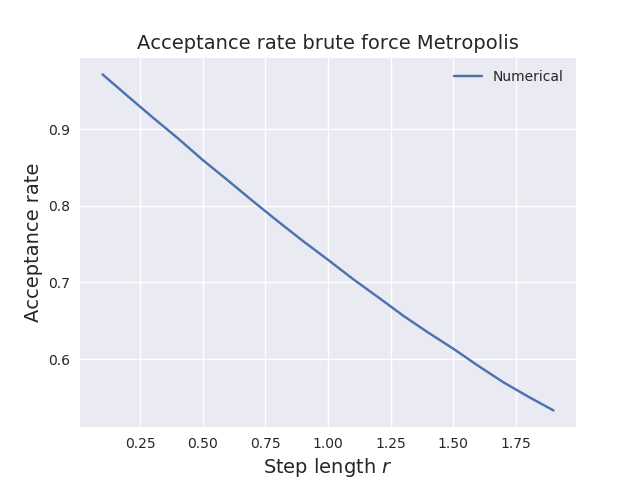
\includegraphics[scale=0.65]{images/acceptance_BF.png}
	\caption{Acceptance ratio for different choices of the stepsize used in the brute force algorithm}
	\label{fig:acceptance_BF_stepsize}
\end{figure} 

\subsubsection{Importance sampling dependence on timestep}
The acceptance ratio for the importance sampling algorithm as a function of the timestep $\delta t$ is shown in figure \ref{fig:acceptance_IS_timestep}. 

\begin{figure} [H]
	\centering
	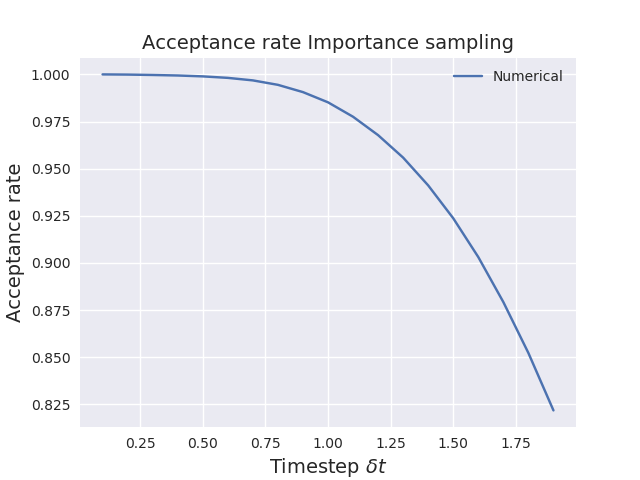
\includegraphics[scale=0.65]{images/acceptance_IS.png}
	\caption{Acceptance ratio for different choices of the timestep $\delta t$  with the Metropolis-Hastings algorithm.}
	\label{fig:acceptance_IS_timestep}
\end{figure} 


\subsection{Variance calculation}

In table \ref{tab:variance_analysis}, we present the results of the local energy calculation with proper error evaluation of statistical error. The statistical error as found with the Blocking method is also compared to the simple way of approximating the variance with equation \ref{eq:variance_simplified}. 

\begin{table} [H]
	\caption{The local energy calculated for $a=0$  without hard-sphere interaction with the Metropolis-Hastings algorithm with analytical local energy calculation, this time with proper evaluation of the statistical error.  The calculations are run in three dimensions with $1e6$ Monte Carlo cycles, and the variational paramameter $\alpha=0.5$}
	\begin{tabularx}{\textwidth}{X|XXXX} \hline
		\label{tab:variance_analysis}
		$N$ & $\langle E_L\rangle$ [$\hbar\omega_{HO}$] & $\sigma^2$ Blocking & $\sigma^2 \approx \langle E_L^2 \rangle - \langle E_L \rangle^2$ \\ \hline
				1 & 1.5000 & 5.0102e-2  & 5.0100e-2 \\
				10 & 15.000 & 4.9701e-1 & 4.9678e-1  \\
				100 & 150.00 & 5.2417 & 5.2184\\
				500 & 750.00 & 9.0710 & 8.4831 \\ \hline
	\end{tabularx}
\end{table}

\subsection{VMC with repulsive interaction}
In table \ref{tab:EL_calc_repulsive_pot}, the results from the calculation of the elliptical trap are presented. The variational parameter $\alpha$ was varied manually to find the minimum of the local energy $E_L$.

\begin{table} [H]
	\centering
	\caption{The local energy $E_L$ calculated for different $\alpha$, with $a=0.0043$  with hard-sphere interaction,  elliptical trap and $\beta=2.82843$, with the brute force algorithm with analytical local energy calculation. We compare the VMC results to the results found by the Gross-Pitaevskii equation (GP) for 1, 10 and 100 particles. The calculations are run in three dimensions with $1e6$ Monte Carlo cycles}
	\begin{tabularx}{\textwidth}{X|XXXXXX} \hline
		\label{tab:EL_calc_repulsive_pot}
		& \multicolumn{2}{c}{\textbf{N=1}} & \multicolumn{2}{c}{\textbf{N=10}} & \multicolumn{2}{c}{\textbf{N=100}} \\
		$\alpha$ & VMC & GP & VMC & GP & VMC & GP  \\ \hline
		0.2 & 3.48489 & 3.50060 & 35.0915 & 35.0060 & 413.853 & 350.060\\
		0.3 & 2.73719 & 2.73611 & 27.5577 & 27.3611 & 359.313 & 273.611\\
		0.4 & 2.47403 & 2.47457 & 24.8541 & 24.7457 & 354.602 & 247.457\\ 
		0.5 & 2.41422 & 2.41421 & 24.2644 & 24.1421 & 371.025 & 241.421\\ 
		0.6 & 2.45456 & 2.45445 & 24.6661 & 24.5445 & 395.560 & 245.445\\ 
		0.7 & 2.55036 & 2.55217 & 25.6275 & 25.5217 & 425.227 & 255.217\\ 
		0.8 & 2.69082 & 2.68581 & 26.8884 & 26.8581 & 457.480 & 268.581\\ \hline
	\end{tabularx}
\end{table}

\subsubsection{Gradient Decent} \label{sec:gd}
The gradient decent method was then used to find the minimum of the local energy in the interacting case. The results are presented in table \ref{tab:EL_calc_gradientdecent}.

\begin{table} [H]
	\centering
	\caption{The local energy $E_L$ calculated with the gradient decent method, with $a=0.0043$  with hard-sphere interaction,  elliptical trap and $\beta=2.82843$, with the brute force algorithm with analytical local energy calculation. The table shows the optimal $\alpha$ found by the method, and the resulting local energy. The calculations are run in for  three dimensions with $1e6$ Monte Carlo cycles.}
	\begin{tabularx}{\textwidth}{X|XXX} \hline
		\label{tab:EL_calc_gradientdecent}
		$N$ & $\alpha $ & $E_L$  & $|\partial E_L/\partial \alpha|$   \\ \hline
		1   & 0.50000  & 2.4142  &  7.2134e-06 \\
		10  & 0.50015  & 24.264  &  4.7969e-05 \\ 
		100 & 0.53379  & 379.39  &  4.1789e-03 \\ \hline
	\end{tabularx}
\end{table}

\iffalse
\subsubsection{Wave function} \label{sec:wf}
Now as we have found the optimal $\alpha$'s for 1, 10 and 100 particles in an elliptical trap, we can plot the respective wave functions. In figure \ref{fig:wf} the wave functions are plotted as a function of the spread in x-direction (dashed lines) in addition to the ideal wave function in a spherical trap (solid line). The results are comparable to earlier publications (see for instance Ref.\cite{Dalfovo}), and show that the wave functions get a broader shape when particles are added.
\begin{figure} [H]
    \centering
    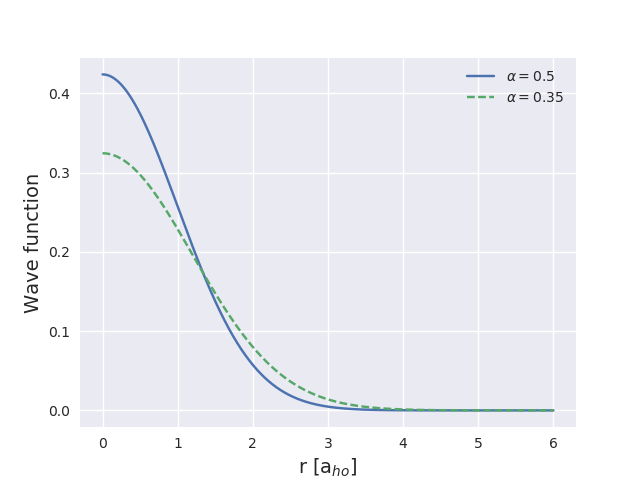
\includegraphics[scale=0.80]{images/wavefunctions.png}
    \caption{The single particle wave functions for a ideal bose gas (solid line) in a spherical harmonic oscillator and for 1, 10 and 100 particles in a elliptical harmonic oscillator (dashed lines). The normalization constant $A=(8\alpha^3/\pi^2\beta)^{1/4}$ is used such that the curvatures are normalized to 1.}
    \label{fig:wf}
\end{figure}
\fi

\subsubsection{Onebody density}
In section \ref{sec:OB_theory} we presented a couple of ways computing the onebody density. Because both should give the same result, we selected the simplest one, which is the method with the bins. We conduct the investigations in elliptic traps, with 10 particles, 3 dimensions and 1e6 Monte Carlo cycles. With the optimal parameter $\alpha$ for the ground state wave function and for both the interacting and the non-interacting case, the onebody density plot is found in figure \ref{fig:ob0}.

\begin{figure} [H]
    \centering
    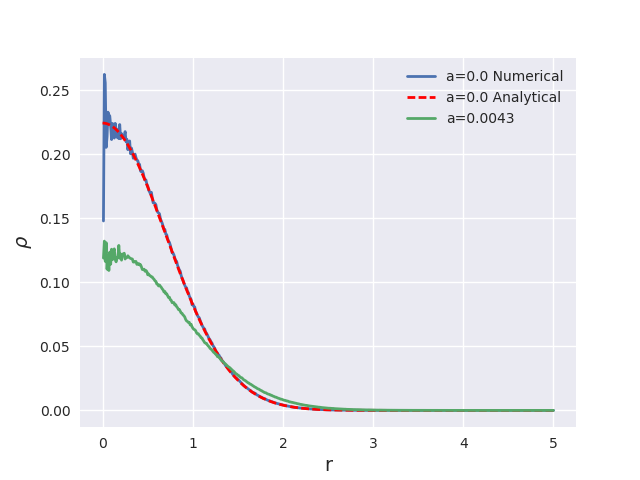
\includegraphics[scale=0.80]{images/ob.png}
    \caption{The onebody density of the bosonic system, which is run with $\alpha=0.5$ for $a=0$ and compared with the analytical expression. The optimal $\alpha$ for the interacting case with $a=0.0043$ was found to be $\alpha = 0.3450$. The radius is given in units of a$_{ho}$ along the x-axis, and the density is in units of a$_{ho}^{-3}$.}
    \label{fig:ob0}
\end{figure}

From the onebody density plot, we observe that the experimental onebody density matches the exact without interacting, and the half peak value is $\sim 0.8$. For the case with interaction, the peak is obviously lower, and we observe a half peak value of $\sim 1.0$, which makes it broader.

\section{Discussion} \label{Discussion}
For the case without interaction and spherical harmonic oscillator we see from figure \ref{fig:EL_as_func_of_alpha} that the minimum of the local energy is found when the varitional parameter $\alpha=0.5$. We also observe that $\alpha=0.5$ gives the minimal variance, and seen from figure \ref{fig:variance_EL_as_func_of_alpha}. The local energy and the variance explode when $\alpha$ is approaching zero.  
\par 
\vspace{3mm}

When comparing the results from the brute force Monte Carlo calculation with spherical harmonic oscillator and no interaction, as shown in table \ref{tab:BFmet}, we observe that in the case when we use an analytical expression for $E_L$, the simulation results yields the exact energy, as obtained from equation \ref{eq:Energy_exact}. Also the numerically calculated $E_L$, as described in section \ref{Numerical_calc_E_L}, reproduces the exact answers with the same presicion as the analytical. 

Moreover, when comparing the CPU time difference between these two calculations, the numerically calculated $E_L$ spends much more time on the calculations compared to the analytically calculated $E_L$-case. The reason for this is probably the numerical differentiation mentioned in equation \ref{eq:num_derv}, which in addition will cause some minor errors. The time difference is as large as a factor of $10^3$ for the 500 particles, three dimensions case. which makes it preferable to use the analytically calculated $E_L$ in our calculations. However, not all trial wave functions $\Psi_T$ or Hamiltonians H will yield an $E_L$ which is analytically possible to calculate, and in this case, one should have a functioning algorithm for numerical calculation of $E_L$ as well.
\par 
\vspace{3mm}

When comparing the results from the brute force and Metropolis-Hastings algorithms, shown in tables \ref{tab:BFmet} and \ref{tab:ISmet}, the reader can observe that the Hastings algorithm reproduces the exact energies, as the brute force algorithm does, but that the Hastings algorithm is slightly slower. This slight time increase is due to the fact that while the brute force algorithm picks a proposed new step at random, the Hasting algorithm makes a more educated move by calculating the drift force $F$ on the particle, and decide what direction the particle is most likely to move in, as described in section \ref{Importance_sampling}. While this calculation spends slightly more CPU time, it is rewarded by the Hastings algorithm having a higher acceptance rate of the proposed moves compared to the brute force Metropolis. This can be seen from figures \ref{fig:acceptance_BF_stepsize} and \ref{fig:acceptance_IS_timestep}. The acceptance ratio of the Hastings algorithm for a timestep $\Delta t=1$ is much higher than the acceptance ratio for brute force with a stepsize $r=1$. This results in the Hastings algorithm moving faster towards the minima compared to the brute force method. This effect, however, is not that visible in our project, but can make a vital difference for larger Monte Carlo simulations.
\par 
\vspace{3mm}

Still studying figure \ref{fig:acceptance_IS_timestep} and \ref{fig:acceptance_BF_stepsize}, we observe that the importance sampling algorithm has a high acceptance rate for intermediate timesteps $\Delta t$, but the acceptance rate drops seemingly exponentially for higher timesteps. Comparing this to the brute force acceptance rate, the drop in the acceptance rate is more like a lineary decreasing curve. This is because the acceptance probability for brute force to do a step in the "wrong direction" is still present, while moving in the wrong direction with importance sampling is much less probable, and therefore the acceptance rate decreases rapidly with increased timestep.
\par 
\vspace{3mm}

In table \ref{tab:variance_analysis}, we repeated the calculation of the no interaction spherical potential with importance sampling, but this time we included a proper evaluation of the error. We compared the variances obtained from the simple, but incorrect way of calculating error, as shown in equation \ref{eq:variance_simplified} to a proper variance calculation using the blocking method, by evaluation equation \ref{eq:sample_var_all_exp}. As expected, the simplified variance calculation underestimates the statistical error, as it does not include the covariance term in equation \ref{eq:sample_var_all_exp}. However, the deviation between the two is small for few number of particles. We would say that as blocking is a quick way of calculating the statistical error, it should be done when presenting results, but the simplified error calculation could still give a quick estimation of the magnitude of the variance in a simulation.
\par 
\vspace{6mm}


Further we have seen that we get som differences between the variational Monte Carlo and the Gross-Pitaevskii calculations. Gross-Pitaevskii (GP) only holds for dilute bose gases, and since the gas gets less dilute the more particles we add, we will expect some deviations when the number of particles increase. Nonetheless, for the interacting case we study a maximum of 100 particles, so this should be a small effect, and we expect the exact GP equation to be accurate for our case. Anyway, we have not solved GP for the interacting case, so the GP benchmark should underestimate the obtained energy, which is also the case.

We can also compare the results to Ref.\cite{DuBois}, where they have plotted energy per particle as a function of number of particles. According to that plot, the energy per particle should increase rapidly when particles are added to a small number of particles, something that we also observe when going from 10 to 100 particles and partly when going from 1 to 10 particles. The exact energy difference is though hard to read from the graph, but our energies are possibly a bit larger than they should be.
\par
\vspace{3mm}

We find the optimal $\alpha$ using gradient descent, and the results match the results obtained when running for various $\alpha$'s, see table \ref{tab:EL_calc_repulsive_pot} and \ref{tab:EL_calc_gradientdecent}. The optimal $\alpha$ tends to increase when adding particles, which complements the observation in \cite{Nilsen}. This is not surprising, since the optimal wave function should change when adding particles with interaction. What value one obtains as the optimal $\alpha$ will be dependent on whether if one starts with an overestimated or an underestimated guess, and we have therefore tried both and decreased the step length $\eta$ to achieve an accurate optimal $\alpha$ with a flat slope. 
\par 
\vspace{3mm}

For the onebody density plots we saw that the densities had gaussian shapes, which come from the wave functions. The peak decreased when adding interaction because the bosons then are more spread out, which also is the reason why it gets broader. We observed noise for small radii, which is caused by the dividing on sphere surfaces, which are small numbers for small radii. All particles are located within a distance $3a_{HO}$ from particle $i$, which makes sence since we only study 10 particles. 


\section{Conclusion}

In this project, we have found that the Variational Monte Carlo method reproduces analytical calculations for the spherical harmonic oscillator without interparticle interaction. The minimum in the energy was found for this case to be $\alpha=0.5$, which is as expected. Both the brute force method with an analytically calculated for $E_L$ and the Hastings algorithm were quick and accurate, while the brute force method with a numerically calculated $E_L$ was much slower.

The Hastings algorithm had a higher acceptance rate for the proposed moves in the Monte Carlo iterations compared to the brute force method. This should result in the Hastings method converging faster, although we did not observe that in this report. We also saw that the Hastings algorithm was more dependent on the timestep compared to the brute force method's dependence om stepsize. This is as we would expect from theory.  \par
When including a proper evaluation of the error by using the blocking method, we saw that the blocking method gave a slightly higher estimated variance, compared to the estimation from equation \ref{eq:variance_simplified}. This is as expected.

ALSO HERE WE NEED TO MENTION THE INTERACTING CASE

Despite the noise seen for onebody density, the non-interacting calculation matched the exact expression pretty well. The particles also spread out when adding repulsive interaction, which is highly expected. 




\newpage
\section{References}
\begingroup
\renewcommand{\section}[2]{}
\begin{thebibliography}{}
	\bibitem{MHJ15}
	Morten Hjorth-Jensen.
	Computational Physics 2: Variational Monte Carlo methods, Lecture Notes Spring 2018.
	Department of Physics, University of Oslo,
	(2018).
	\bibitem{DuBois}
	J. L. DuBois and H. R. Glyde, H. R., \emph{Bose-Einstein condensation in trapped bosons: A variational Monte Carlo analysis}, Phys. Rev. A \textbf{63}, 023602 (2001).
	\bibitem{Nilsen}
	J. K. Nilsen,  J. Mur-Petit, M. Guilleumas, M. Hjorth-Jensen, and A. Polls, \emph{Vortices in atomic Bose-Einstein condensates in the large-gas-parameter region}, Phys. Rev. A \textbf{71}, 053610, (2005).
	\bibitem{Dalfovo}
	F. Dalfovo, S. Giorgini, L. P. Pitaevskii, S. Stringari, \emph{Theory of Bose-Einstein condensation in trapped gases} Rev. Mod. Phys. \textbf{71}, 463, (1999).
	\bibitem{JE2016}
	J. Emspak, \emph{States of Matter: Bose-Einstein Condensate}, LiveScience, (2016).
	\url{https://www.livescience.com/54667-bose-einstein-condensate.html}
	Downloaded March 15th 2018.
	\bibitem{SP}
	S. Perkowitz \emph{Bose-Einstein condensate} Encyclopaedia Britannica 
	\url{https://www.britannica.com/science/Bose-Einstein-condensate}
	Downloaded March 15th 2018.
	\bibitem{Anderson}
	    M. H. Anderson, J. R. Ensher, M. R. Matthews, C. E. Wieman, E. A. Cornell, \emph{Observation of Bose-Einstein Condensation in a Dilute Atomic Vapor}, Science \textbf{269}, (1995).
	\bibitem{JKNilsen}
		J. K. Nilsen \emph{Bose-Einstein condensation in trapped bosons: A quantum Monte Carlo analysis}, Master thesis 2004, Department of Physics, University of Oslo, (2004). 
	\bibitem{Gross}
		E. P. Gross, \emph{Structure of a quantized vortex in boson systems}, Il Nuovo Cimento, \textbf{20} (3): 454–457, (1961).
	\bibitem{Pitaevskii}
		 L. P. Pitaevskii, \emph{Vortex lines in an imperfect Bose gas}, Sov. Phys. JETP. \textbf{13} (2): 451–454, (1961).

	
\end{thebibliography}
\endgroup

\newpage

\section*{Appendix A} \label{appendix_A}
In the theory section we presented the analytical expressions for the local energy, and in this appendix we go though the derivations carefully for those of you who are curious. Firstly we present the local energies where we ignore the two-particle interaction, and we also focus on the spherical harmonic oscillator trap since we do not look at the elliptical trap without interaction, even though the expressions are similar.

Secondly the general expression which can be used with and without interaction, with spherical or elliptical harmonic oscillator trap and with a various number of parameter values is derived. This can in principle be used for every case, but it is more complex than the special ones where we ignore interaction and we therefore expect it to be slower. 

\subsection{Without repulsive interaction}
We calculated the analytical expression for the local energy $E_L$, as given by \ref{eq:Local_energy}, for the non-interaction ($a=0$) case for the spherical harmonic oscillator. In this case, the trial wave function only consists of the one body part, and is thus for $N$ particles given by:

\begin{equation}
	\label{eq:WF_nointeract}
	\Psi_T(\vec{r}) = \prod_i^N e^{-\alpha(x_i^2 + y_i^2 + \beta z_i^2)}
\end{equation}

We now want to calculate the analytical expressions for $E_L$ for one particle and one dimension, and $N$ particles and three dimensions.

\subsubsection{One particle, one dimension}

From equation \ref{eq:WF_nointeract}, the trial wave function for one particle and one dimension is as follows:

\begin{equation}
	\label{eq:WF_1dim_1N}
	\Psi_T(x) = e^{-\alpha x^2} 
\end{equation}
We start from the local energy equation in equation \ref{eq:Local_energy}, where we need to take the second derivative
\begin{align}
\frac{d\Psi_T}{dx}&=-2\alpha xe^{-\alpha x^2}\\
\frac{d^2\Psi_T}{dx^2}&=-2\alpha e^{-\alpha x^2}+4\alpha^2x^2e^{-\alpha x^2}.
\end{align}
To get a neat expression, we use the dimensionless Hamiltonian with spherical harmonic oscillator potential, from equation \ref{eq:Hamilton}, and obtain
\begin{align}
E_L(\alpha)&=-\frac{1}{2}(-2\alpha + 4\alpha^2x^2)+\frac{1}{2}x^2\notag\\
&=\alpha+\Big(\frac{1}{2}-2\alpha^2\Big)x^2
\end{align}

\iffalse
In the Hamiltonian, the Laplace-operator reduces to the partial derivative in the x-direction, $\frac{\partial^2 }{\partial x^2}$, and $E_L$ is 

\begin{equation}
\begin{aligned}
E_L(x) &=  \frac{1}{\Psi_T(x)}\hat{H}\Psi_T(x) \\ 
			 & =  e^{\alpha x^2} (-\frac{\hbar^2}{2m}\frac{\partial^2 }{\partial x^2} + \frac{1}{2} m \omega_{HO}^2 x^2) e^{-\alpha x^2}  \\
			 & = e^{\alpha x^2} [-\frac{\hbar^2}{2m}\frac{\partial^2 }{\partial x^2} (e^{-\alpha x^2}) + \frac{1}{2} m \omega_{HO}^2 x^2 (^{-\alpha x^2})]
\end{aligned}
\end{equation}

Double differentiation of $ e^{-\alpha x^2}$ yields

\begin{equation}
\frac{\partial^2}{\partial x^2} (e^{-\alpha x^2}) = e^{-\alpha x^2} 2 \alpha (2x^2 -1)
\end{equation}

Inserting this into the expression for $E_L$ gives

\begin{equation}
E_L(\alpha) = -\frac{\hbar^2}{m} \alpha (2x\alpha^2 -1) + \frac{1}{2} m\omega_{HO}^2x^2
\end{equation}
\fi

\subsubsection{$N$ particles, three dimensions}

When extending the non-interaction case to $N$ particles and three dimensions, the trial wave function will take the form listed in equation \ref{eq:WF_nointeract}, and the Hamiltonian will be as listed in equation \ref{eq:Hamilton} with the dimensionless spherical harmonic oscillator potential $\frac{1}{2}r_i^2$, as listed in \ref{eq:V_ext}.

\iffalse
The local energy is then

\begin{equation}
	E_L(\alpha) = \prod_i^N e^{\alpha(x_i^2 + y_i^2 + \beta z_i^2)} \sum_i [ -\frac{\hbar^2}{2m} \nabla_i^2 + \frac{1}{2}m\omega_{HO}^2(x_i^2 + y_i^2 + z_i^2)] \prod_i^N e^{-\alpha(x_i^2 + y_i^2 + \beta z_i^2)}
\end{equation}

Double differentiation of $\Psi_T$ with respect to x gives

\begin{equation}
	\frac{\partial^2}{\partial x^2} (\prod_i e^{-\alpha(x_i^2 + y_i^2 + \beta z_i^2)}) = \prod_i e^{-\alpha(x_i^2 + y_i^2 + \beta z_i^2)} [\sum_{i,j} 4 \alpha^2 x_i x_j -2 \alpha N ]
\end{equation}

Double differentiation with respect to y will give similar answer, while for z there will be a factor $\beta$ difference

\begin{equation}
\frac{\partial^2}{\partial z^2} (\prod_i e^{-\alpha(x_i^2 + y_i^2 + \beta z_i^2)}) = \prod_i e^{-\alpha(x_i^2 + y_i^2 + \beta z_i^2)} [\sum_{i,j} 4 \alpha^2 \beta^2 y_i y_j -2 \alpha \beta N ]
\end{equation}

By including the answers from the differentiations in the x,y and z directions and simplifying the expression results in the following expression for the local energy \textcolor{red}{hvor er $\beta$ i denne utregningen?}

\begin{equation}
\begin{aligned}
	E_L(\alpha) & = -\frac{\hbar^2}{2m} N [ \sum_{i,j} 4 \alpha^2 x_i x_j + \sum_{i,j} 4 \alpha^2 y_i y_j + \sum_{i,j} 4 \alpha^2 \beta^2 z_i z_j] +  \\ & \frac{2 \hbar^2}{m}\alpha N^2 + \sum_i \frac{1}{2}m\omega_{HO^2}(x_i^2 + y_i^2 + z_i^2) + \frac{\hbar^2}{m}\beta \alpha N^2
\end{aligned}
\end{equation}
\fi


For this case it might be better to use spherical coordinates, where the Laplace operator is given by
\begin{equation}
\nabla^2=\frac{1}{r^2}\frac{\partial}{\partial r}\bigg(r^2\frac{\partial}{\partial r}\bigg)
\end{equation}
when we only take the radial part into account. We transform the wavefunction from a product to a function with a sum in the exponent, and calculate the first derivative
\begin{equation}
\frac{\partial\Psi_T}{\partial r_j}=-2\alpha r_j \exp\bigg[-\alpha\bigg(\sum_i r_i^2\bigg)\bigg].
\end{equation}
After adding a $r_j^2$, we differentiate the expression again
\begin{equation*}
\frac{\partial}{\partial r_j}\bigg(-2\alpha r_j^3\exp\Big[-\alpha\Big(\sum_i r_i^2\Big)\Big]\bigg)
=(-6\alpha r_j^2 + 4\alpha^2r_j^4)\exp\Big[-\alpha\Big(\sum_i r_i^2\Big)\Big]
\end{equation*}
and we obtain
\begin{equation}
\frac{\nabla_j^2\Psi_T}{\Psi_T}=-6\alpha+4\alpha^2r_j^2.
\end{equation}
Again we get the local energy from the Hamiltonian with a spherical harmonic oscillator potential. 
\begin{align}
E_L(\alpha)&=\sum_j-\frac{1}{2}(-6\alpha+4\alpha^2r_j^2) + \frac{1}{2}r_j^2\notag\\
&=3N\alpha + \Big(\frac{1}{2}-2\alpha^2\Big)\sum_{j=1}^Nr_j^2
\end{align}

\subsubsection{General}
If one now studies the local energy expressions for one particle in one dimension and $N$ particles in three dimensions, one can see a pattern and it is easy to imagine that there exists a general expression for the local energy, when interaction is ignored and for the spherical harmonic oscillator case. At least for 1, 2, and 3 dimensions, it can be shown that 
\begin{equation}
E_L(\alpha)=dim\cdot N\cdot \alpha+\Big(\frac{1}{2}-2\alpha^2\Big)\sum_{j=1}^Nr_j^2.
\end{equation}
A similar expression for the elliptical trap can be found to be
\begin{equation}
E_L(\alpha)=2\alpha+\alpha\beta+\Big(\frac{1}{2}-2\alpha^2\Big)\sum_{j=1}^Nr_j^2.
\end{equation}
in three dimensions.

\subsection{With repulsive interaction}
As mentioned in the theory section, the calculations get more complicated when adding the interaction, and we are in fact not able to find the local energy analytically. However, we can simplify the local energy expression and hopefully gain some speed up compared to when we do all the calculations numerically. 

We start with defining the onebody part of the wavefunction as $\Phi$ and the Jastrow factor as $\exp\big(u(r_{ij})\big)$ such that the total trial wavefunction becomes
\begin{equation}
\Psi_T(\vec{r}_1,\hdots\vec{r}_N)=\Big[\prod_i\Phi(\vec{r}_i)\Big]\exp\Big(\sum_{i<j}u(r_{ij})\Big)
\end{equation}

Thereafter we calculate the term connected to the kinetic part of the Hamiltonian,
\begin{equation}
\frac{\nabla_k^2\Psi_T(\vec{r})}{\Psi_T(\vec{r})},
\label{eq:ham_kin}
\end{equation}
which is the most difficult part. We apply the product rule and obtain the following expression for the first derivative
\begin{align}
\nabla_k\Psi_T(\vec{r})&=\nabla_k\Phi(\vec{r}_k)\Big[\prod_{i\neq k}\Phi(\vec{r}_i)\Big]\exp\Big(\sum_{i<j}u(r_{ij})\Big)\notag\\
&\phantom{=}+\prod_i\Phi(\vec{r}_i)\exp\Big(\sum_{i<j}r(r_{ij})\Big)
\sum_{j\neq k}\nabla_k u(r_{ij})
\end{align}

For the second derivative we get five terms in total where two of them are cross terms and therefore equal. 
\begin{align}
\nabla_k^2\Psi_T(\vec{r})&=\nabla_k^2\Phi(\vec{r}_k)\Big[\prod_{i \neq k}\Phi(\vec{r}_i)\Big]\exp\Big(\sum_{i<j}u(r_{ij})\Big)\notag\\
&\phantom{=}+\nabla_k\Phi(\vec{r}_k)\Big[\prod_{i \neq k}\Phi(\vec{r}_i)\Big]\exp\Big(\sum_{i<j}u(r_{ij})\Big)\sum_{j\neq k}\nabla_ku(r_{ij})\notag\\
&\phantom{=}+\nabla_k\Phi(\vec{r}_k)\Big[\prod_{i \neq k}\Phi(\vec{r}_i)\Big]\exp\Big(\sum_{i<j}u(r_{ij})\Big)\sum_{j\neq k}\nabla_ku(r_{ij})\\
&\phantom{=}+\prod_i\Phi(\vec{r}_i)\exp\Big(\sum_{i<j}u(r_{ij})\Big)\sum_{i\neq k}\nabla_ku(r_{ij})\sum_{j\neq k}\nabla_ku(r_{ij})\notag\\
&\phantom{=}+\prod_i\Phi(\vec{r}_i)\exp\Big(\sum_{i<j}u(r_{ij})\Big)\sum_{j\neq k}\nabla_k^2u(r_{ij})\notag
\end{align}
To simplify this, we do a change of variables
\begin{equation}
\frac{\partial}{\partial \vec{r}_k}=\frac{\partial}{\partial \vec{r}_k}\frac{\partial r_{kj}}{\partial r_{kj}}=\frac{\partial r_{kj}}{\partial \vec{r}_k}\frac{\partial}{\partial r_{kj}}=\frac{(\vec{r}_k-\vec{r}_j)}{r_{kj}}\frac{\partial}{\partial r_{kj}}
\end{equation}
where we have used that
\begin{equation}
\frac{\partial r_{kj}}{\partial \vec{r}_k}=\frac{\vec{r}_k - \vec{r}_j}{|\vec{r}_k - \vec{r}_j|}=\frac{\vec{r}_k - \vec{r}_j}{r_{kj}}.
\end{equation}
In addition we need to differentiate $u(r_{ij})$ once and twice
\begin{equation}
\nabla_ku(r_{ij})=\frac{\partial r_{kj}}{\partial \vec{r}_k}\frac{\partial}{\partial r_{kj}}\big(u(r_{ij})\big)=\frac{\vec{r}_k - \vec{r}_j}{|\vec{r}_k - \vec{r}_j|}u'(r_{kj})
\end{equation}
\begin{align*}
\nabla_k^2u(r_{ij})&=\nabla_k\bigg(\frac{\vec{r}_k - \vec{r}_j}{|\vec{r}_k - \vec{r}_j|}u'(r_{kj})\bigg)\\
&=\frac{1}{|\vec{r}_k-\vec{r}_j|}\frac{\partial}{\partial r_{kj}}\big(u(r_{kj})\big)+\frac{\partial^2}{\partial r_{kj}^2}\big(u(r_{kj})\big)\\
&\phantom{=}+\frac{(\vec{r}_k-\vec{r}_j)(\vec{r}_k-\vec{r}_j)}{|\vec{r}_k-\vec{r}_j|^3}\frac{\partial}{\partial r_{kj}}\big(u(r_{kj})\big)
\end{align*}
where we can simplify the last term
\begin{equation}
\frac{(\vec{r}_k-\vec{r}_j)(\vec{r}_k-\vec{r}_j)}{|\vec{r}_k-\vec{r}_j|^3}=\frac{(\vec{r}_k - \vec{r}_j)(\vec{r}_k - \vec{r}_j)}{(\vec{r}_k - \vec{r}_j)(\vec{r}_k - \vec{r}_j)|\vec{r}_k - \vec{r}_j|}=\frac{1}{|\vec{r}_k - \vec{r}_j|}.
\end{equation}
Finally we can write out the expression from equation (\ref{eq:ham_kin}) 
\begin{align}
\frac{\nabla_k^2\Psi_T}{\Psi_T}&=\frac{\nabla_k^2\Phi(\vec{r}_k)}{\Phi(\vec{r}_k)} + 2\frac{\nabla_k\Phi(\vec{r}_k)}{\Phi(\vec{r}_k)}\bigg(\sum_{j\neq k}\frac{(\vec{r}_k-\vec{r}_j)}{r_{kj}}u'(r_{kj})\bigg)\notag\\
&\phantom{=}+\sum_{ij\neq k}\frac{(\vec{r}_k-\vec{r}_j)(\vec{r}_k-\vec{r}_j)}{r_{kj}r_{ki}}u'(r_{kj})u'(r_{ki})\\
&\phantom{=}+\sum_{j\neq k}\bigg(\frac{(\vec{r}_k-\vec{r}_j)}{r_{kj}}u''(r_{kj})+\frac{2}{r_{kj}}u'(r_{kj})\bigg)\notag
\end{align}
Now we can easily find a local energy expression using the general expression for the local energy:
\begin{align}
E_L&=\frac{1}{\Psi_T}\bigg(\sum_i\Big(-\frac{1}{2}\nabla_i^2+V_{ext}(\vec{r}_i)\Big) + \sum_{i<j}V_{int}(\vec{r}_i,\vec{r}_j)\bigg)\Psi_T\notag\\
&=\sum_i\Big(-\frac{\nabla_i^2\Psi_T}{2\Psi_T}+V_{ext}(\vec{r}_i)\bigg)+\sum_{i<j}V_{int}(\vec{r}_i,\vec{r}_j)
\end{align}

\section*{Appendix B} \label{sec:appendix_b}

This section shows the analytical calculations for the drift force $F$, as given by equation \ref{eq:drift_force} for the non-interaction case.

\subsubsection{$N$ particles, 1 dimension}

The no interaction, N particle trial wave function $\psi_T$ is given by

\begin{equation}
\psi_T =	\prod_i e^{-\alpha x_i^2}
\end{equation}
The drift force F is then

\begin{align}
	F = \frac{2 \nabla ( \prod_i e^{-\alpha x_i^2} )}{ \prod_i e^{-\alpha x_i^2} }
\end{align}

The differentiation $\nabla \rightarrow \frac{d }{d x}$, as we operate in one dimension. The differentiation of $\psi_T$ yields

\begin{equation}
	\label{eq:differentiation_WF}
	\frac{d}{d x} \Big( \prod_i e^{-\alpha x_i^2}\Big) =  \prod_i e^{-\alpha x_i^2} \sum_i (-2\alpha x_i)
\end{equation}

This yields the drift force $F$

\begin{equation}
	F =  2\cdot \prod_i e^{\alpha x_i^2}   \prod_i e^{-\alpha x_i^2} \sum_i (-2\alpha x_i) = - 4 \alpha \sum_i x_i
\end{equation}

\subsubsection{$N$ particles, 3 dimensions}

In the $N$ particles, $3$ dimensions case, the trial wave function $\psi_T$ takes the following form

\begin{equation}
	\psi_T = \prod_i e^{- \alpha (x_i^2 + y_i^2 + \beta z_i^2)} 
\end{equation}

As we operate in three dimensions, $\nabla = (\frac{d}{dx}, \frac{d}{dy}, \frac{d}{dy})$. The differentiation in one dimension of $\psi$ is shown in equation \ref{eq:differentiation_WF}, and the results are similar for the differentiation with respect to $y$ and $z$, the only difference being an extra factor $\beta$ in the expression for $\frac{d \psi_T}{d z}$, due to the $\beta$ in the expression for $\psi_T$. Thus the drift force F for $N$ particles in three dimensions is 

\begin{equation}
	F = -4 \alpha \Big(\sum_i xi, \sum_i y_i, \sum_i \beta z_i \Big)
\end{equation}

\section*{Appendix C} \label{sec:appendix_c}
In the theory part we claimed that the Hamiltonian could be written as
\begin{equation}
H=\sum_i\bigg(\frac{1}{2}\Big(-\nabla^2 + x_i^2 + y_i^2 + \gamma^2z_i^2\Big)\bigg)+\sum_{i<j}V_{int}(\vec{r}_i,\vec{r}_j)
\end{equation}
for an elliptical harmonic oscillator potential with repulsive interaction. Let us start from scratch, where the unscalled Hamiltonian for an elliptical harmonic oscillator reads
\begin{equation*}
H=\sum_i\bigg(-\frac{\hbar^2}{2m}\nabla_i^2+\frac{1}{2}m\Big(\omega_{HO}^2(x_i^2+y_i^2)+\omega_z^2z_i^2\Big)\bigg)+\sum_{i<j}V_{int}(\vec{r}_i, \vec{r}_j).
\end{equation*}
We then scale the entire equation with respect to $\hbar\omega_{HO}$
\begin{equation*}
\frac{H}{\hbar\omega_{HO}}=\sum_i\bigg(-\frac{\hbar}{2m\omega_{HO}}\nabla_i^2+\frac{1}{2}\frac{m}{\hbar}\omega_{HO}(x_i^2+y_i^2)+\frac{1}{2}\frac{m}{\hbar}\frac{\omega_z^2}{\omega_{HO}}z_i^2\bigg)+\sum_{i<j}V_{int}(\vec{r}_i, \vec{r}_j)
\end{equation*}
where we can take $H'=H/\hbar\omega_{HO}$ as the dimensionless energy. Further we scale all the lengths in the same way
\begin{equation*}
x_i^2=(x_i')^2\cdot a_{HO}^2=(x_i')^2\cdot\frac{\hbar}{m\omega_{HO}},
\end{equation*}
where we have used the relation $a_{HO}\equiv (\hbar/m\omega_{HO})^{1/2}$, and we finally obtain
\begin{equation}
H'=\sum_i\frac{1}{2}\bigg(-\nabla_i^2+(x_i')^2+(y_i')^2+\frac{\omega_z^2}{\omega_{HO}^2}(z_i')^2\bigg)+\sum_{i<j}V_{int}(\vec{r}_i, \vec{r}_j)
\end{equation}
which is the Hamiltonian that we were hunting. We know how the factor in front of the $z^2$ factor is $\beta^2 = \gamma^2$, so $\beta = \gamma$ has to be equal to $\omega_z/\omega_{HO}$.

\section*{Appendix D} \label{sec:appendix_d}
To check if the VMC results are correct, we need a benchmark, and for a dilute bose gas the Gross-Pitaevskii equation is a natural choice. We could have solved the equation for the interacting case using numerical methods, but it would require significantly more effort and we take care of the non-interacting case instead. We start with the dimensionless brother of equation \ref{eq:GP_integral},
\begin{equation}
E_{\text{GP}}[\Psi]=\int d\vec{r}\bigg[\frac{1}{2}|\nabla\Psi(\vec{r})|^2+V_{ext}(\vec{r})|\Psi|^2+2\pi a|\Psi|^4\bigg].
\end{equation}
where 
\begin{equation}
V_{ext}(\vec{r})=\frac{1}{2}(x_1^2+y_1^2+\beta z_1^2 + \hdots + x_N^2+y_N^2+\beta z_N^2)
\end{equation}
for N particles in an 3D elliptical trap. The normalized wave function without the Jastow factor reads
\begin{equation}
\Psi(\vec{r})=\bigg(\frac{2\alpha}{\pi}\bigg)^{3N/4}\cdot\beta^{N/4}\exp\big(-\alpha(x_1^2+y_1^2+\beta z_1^2 + \hdots + x_N^2+y_N^2+\beta z_N^2)\big).
\end{equation}
This gives us the following expression for the gradient of the wave function squared
\begin{equation}
|\nabla\Psi(\vec{r})|^2=4\alpha^2(x_1^2+y_1^2+\beta^2 z_1^2 + \hdots + x_N^2+y_N^2+\beta^2 z_N^2)|\Psi(\vec{r})|^2.
\end{equation}

Since we ignore the interaction, $a=0$ and we do not need to take the last term into account. The intergral to solve is then
\begin{equation*}
E_{\text{GP}}=\Big(\frac{1}{2}+2\alpha^2\Big)\int_{-\infty}^{\infty}(x_1^2+y_1^2+\beta^2 z_1^2 + \hdots + x_N^2+y_N^2+\beta^2 z_N^2)|\Psi|^2d\vec{r}
\end{equation*}
which is gaussian and can be found in a collection of integrals:
\begin{equation}
\int_{-\infty}^{\infty}e^{-(ax^2+b)}dx=\frac{1}{2a}\sqrt{\frac{\pi}{a}}e^{-b}.
\end{equation}
With some straightforward computations one will find
\begin{align}
E_{\text{GP}}(\alpha,\beta,N)&=\Big(\frac{1}{2}+2\alpha^2\Big)\Big(\frac{2\alpha}{\pi}\Big)^{3N/2}\beta^{N/2}\frac{1}{4\alpha}\sqrt{\frac{\pi}{2\alpha}}^{3N}(2+\beta)\cdot N\cdot \beta^{-N/2}\notag\\
&=N\cdot\Big(\frac{1}{4\alpha}+\alpha\Big)\cdot\Big(1+\frac{\beta}{2}\Big).
\end{align}
This gives the correct analytical results for the non-interacting case both in the spherical trap ($E_L=0.5N\cdot dim$ for $\alpha=0.5$) and the elliptical trap ($E_L=N(1+\beta/2)$\footnote{We start from the exact energy formula for a harmonic oscillator, $E_n=\hbar\omega(n+1/2)$, and study how the ground state energy changes if the z-component has different frequency $\omega_z$ from the other components, $E_0=\hbar(\omega_{ho}+\omega{z}/2)$. If we then scale with respect to $\hbar\omega_z$ as done before, we get $E'=1+\beta/2$ for one particle. For our particular project, we have $\beta=\sqrt{8}$, and get an ground state energy $1+\sqrt{2}$ per particle.} for $\alpha=0.5$ in 3D).

\end{document}
